\documentclass[a4paper]{article}
\usepackage[T1]{fontenc}  			% make sure to install cm-super package for improved PDF quality
\usepackage[utf8]{inputenc}
\usepackage{lmodern}
\usepackage[english]{babel}

%\usepackage[cm]{fullpage}			% Fullpage for now
\usepackage{graphicx}
\usepackage[dvipsnames]{xcolor}
\usepackage[font=small]{caption}
\usepackage{subcaption}
\usepackage{microtype}			 	% microtypographical fine-tunning
\usepackage{setspace} 				% Provides support for setting the spacing between lines in a document.
\usepackage{tocbibind}				% Add bibliography/index/contents to Table of Contents.
\usepackage{mathtools}				% enhances amsmath (no need to load amsmath)
\usepackage{amssymb}
\usepackage{amsfonts}
\usepackage{amsthm}
\usepackage{bm} 					% bold math symbols including greek letters
\usepackage{booktabs}				% professional tables (w/o vertical bars)
\usepackage{array}					% 
\usepackage{dcolumn} 				% align to decimal point in tables
\usepackage[shortcuts]{extdash} 	% hyphenation of dashed words
\usepackage[algoruled]{algorithm2e}
\newcommand\mycommfont[1]{\small\ttfamily #1}
\SetCommentSty{mycommfont}
\usepackage{cleveref}				% clever environment referencing
\crefname{figure}{Fig.}{Figs.}
\crefname{algorithm}{Alg.}{Algs.}
\usepackage{siunitx}				% typesetting of SI units
%\usepackage{paralist}		     	% compact lists with more options
%\usepackage[]{todonotes}			% TODO notes
%\presetkeys{todonotes}{backgroundcolor=orange!50}{}
% Not sure which to use for bibliography
%\usepackage{cite}
%\usepackage{citesort}
\usepackage[square, sort, numbers, authoryear]{natbib}
%\usepackage{pgfplots}


\begin{document}

\section{Euler's Method}\label{sec:euler_method}
It's the simplest method of numerical solution for ordinary differential equations (ODEs).
Suppose we are given the following ODE with and initial condition
\begin{equation}\label{eq:ode}
	y'(t) = f(t, y(t)), \quad y(t_0) = y_0,
\end{equation}
where \( y'(t) = \frac{\mathrm{d}y}{\mathrm{d}t} \) denotes derivative.
Derivatives with respect to time, which are common in physics, are conventionally denoted by the dot symbol. 
That is, \( \dot{y}(t) \equiv y'(t) \equiv \frac{\mathrm{d}y}{\mathrm{d}t} \).
\Cref{eq:ode} is in continuous time \( t \)\footnote{Since this is mathematics we're dealing with, the variable \( t \) does not have to represent time, of course.}.
The solution of the ODE above is a function of time \( y(t) \) for which the above equation holds.
Since we are working with computers, we can't store functions of continuous variable\footnote{Because that would take up infinite memory.} and so we need to discretize the solution.
In other words, we wanna convert it to an equation in discrete time, because it's easier to implement.

The Euler method chooses some finite time step \( h \), so that \( k \)-th discrete time step can be expressed as \( t_k = t_0 + kh \).
One step of the Euler method from \( t_k \) to \( t_{k+1}  = t_k + h \) is given by
\begin{equation}
	y_{k+1} = y_k + hf(t_k, y_k),
\end{equation}
where, obviously, \( y_k = y(t_k) \).
As you can see, the recursion can be started with \( y_0 \) at \( t_0 \), because both of these are given.
We can rewrite the Euler method as 
\begin{equation}
	\frac{y_{k+1} - y_k}{h} = f(t_k, y_k)
\end{equation}

So, for example if my equation for the change in the x-coordinate in the continuous time is given by
\begin{equation}
	\dot{x}(t) = v(t)\cos(\psi(t)),
\end{equation}
than, by application of the Euler method, the discretized version with step size \( h = \mathrm{d}t \) will look like this
\begin{equation}\label{}
	x(t_{k+1}) = x(t_{k}) + v(t_k)\cos(\psi(t_k)) \mathrm{d}t.
\end{equation}
Now, to comport with the notational conventions, we are gonna use the lower index to denote the discre time steps. Since the time steps are only distinguished by the variable \( k \), using variable \( t_k \) is a bit redundant, so we will get rid of it too.
Ultimately, we get
\begin{equation}\label{eq:ode_euler}
	x_{k+1} = x_{k} + v_k\cos(\psi_k) \mathrm{d}t.
\end{equation}

With the help of the Euler method, we have converted a \emph{differential} equation into a \emph{difference} equation.
There are plenty of other, more accurate, methods for ODE integration, such as Runge-Kuta method (see Wikipedia for more), but they are more complicated.



\section{Kinematic Bicycle Model}\label{sec:kinematic_bicycle_model}
This is the kinematic bicycle model
\begin{subequations}
\begin{align}\label{eq:kinematic_bicycle_model_continuous}
\dot{x} 	&=  v \cos(\psi + \beta) \\
\dot{y} 	&=  v \sin(\psi + \beta) \\
\dot{\psi} 	&=  \frac{v}{l_r} \sin(\beta) \\
\dot{v} 	&=  a \\
\dot{\beta} &= \arctan\left(\frac{l_r}{l_r + l_f}\tan(\delta_f)\right)
\end{align}
\end{subequations}
Note, that the Cartesian position \( x,\ y \), the speed\footnote{a.k.a. velocity magnitude} \( v \), the inertial heading angle \( \psi \), the angle of the current velocity \( \beta \), the steering angle \( \delta \triangleq \delta_f \) and acceleration \( a \) are all functions of time.
In ODE speak, these would be called \emph{dependent variables}, whereas \( t \) is the \emph{independent variable}.
Guess why!
The distances from the center of gravity to the rear \( l_r \) axle and to the front \( l_f \) axle are constant parameters, which vary depending on the vehicle.
The \Cref{fig:kinematic_bicycle_model}, stolen from \cite{Kong2015}, depicts the geometric meaning of the variables involved.
\begin{figure}[h]
	\centering
	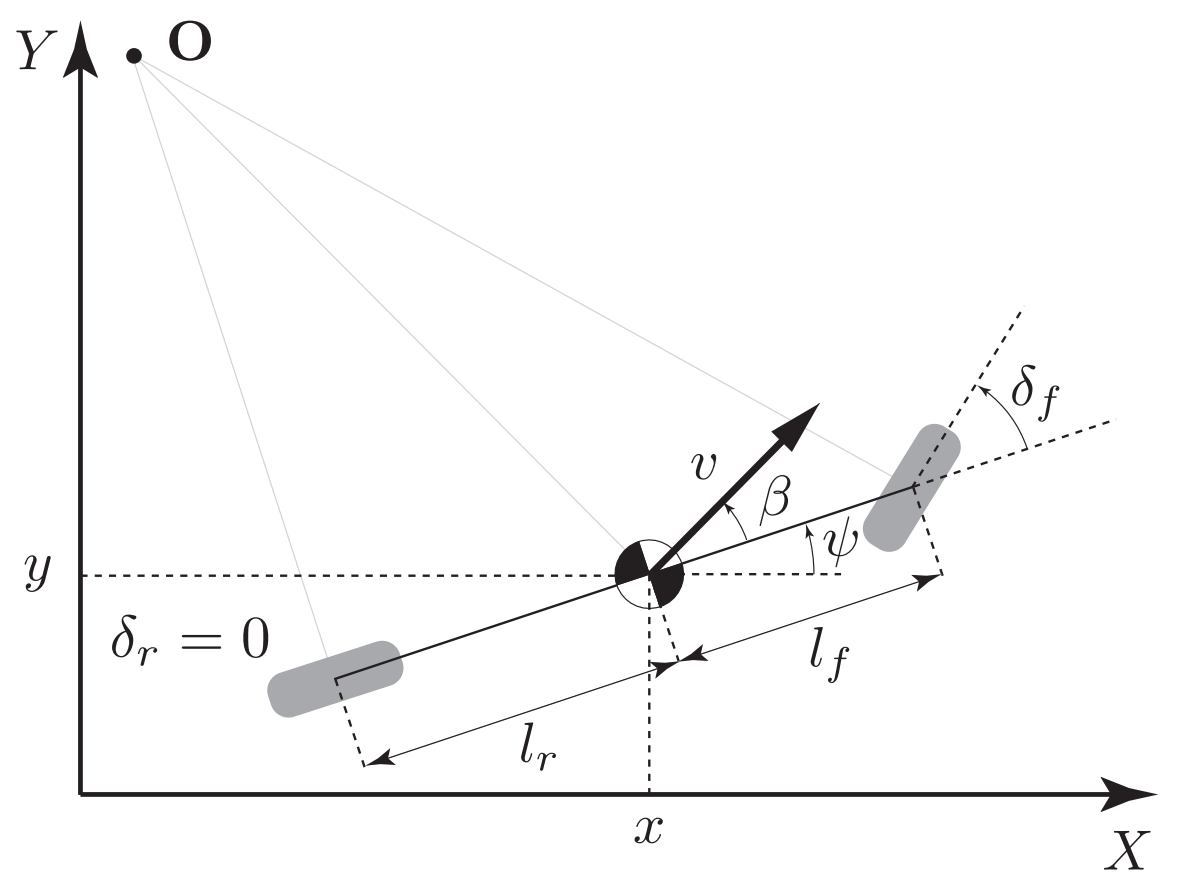
\includegraphics[scale=0.2]{./img/kinematic_bicycle_model.png}
	\caption{Kinematic bicycle model.}
	\label{fig:kinematic_bicycle_model}
\end{figure}

For some undisclosed reason, at Udacity, we are using a simplified version, given by
\begin{subequations}
\begin{align}\label{eq:kinematic_bicycle_model_continuous_udacity}
\dot{x} 	&=  v \cos(\psi) \\
\dot{y} 	&=  v \sin(\psi) \\
\dot{\psi} 	&=  \frac{v}{l_f} \delta \\
\dot{v} 	&=  a \\
\end{align}
\end{subequations}
I guess, this model assumes, among other things, that the velocity vector always points forward (in direction of the longitudinal axis of the vehicle) and the rear axle distance \( l_r = 0 \), but don't quote me on that.
Applying the Euler method from \Cref{sec:euler_method} yields the familiar equations
\begin{subequations}
\begin{align}\label{eq:kinematic_bicycle_model_discrete_udacity}
x_{k+1} 	&= x_k + v_k\cos(\psi_k) \mathrm{d}t \\
y_{k+1} 	&= y_k + v_k\sin(\psi_k) \mathrm{d}t \\
\psi_{k+1} 	&= \psi_k + \frac{v_k}{l_f}\delta_k \mathrm{d}t \\
v_{k+1} 	&= v_k + a_k\mathrm{d}t \\
\end{align}
\end{subequations}
where the \( \mathrm{d}t \) is the discretization step size.
The equations above conform to the nonlinear discrete-time state-space model in the form
\begin{equation}\label{eq:mpc_general_ssm}
	\bm{x}_{k+1} = \bm{f}(\bm{x}_k),\qquad \bm{x}_0
\end{equation}
where the state of the system is given by \( \bm{x}_k = \left[x_k,\ y_k,\ \psi_k,\ v_k \right]^\top \) and \( \bm{f}: \mathbb{R}^4\to\mathbb{R}^4 \) is the system dynamics.
The control vector \( \bm{u}_k = \left[a_k,\ \delta_k\right]^\top \) contains the system inputs; that is, the acceleration \( a_k \) and the steering angle \( \delta_k \), that influence the system state and outputs.




\section{Model Predictive Control}\label{sec:model_predictive_control}
The goal of the controller is to determine optimal values of the control variables at each time step, such that the specified optimality criteria\footnote{Such as, "don't jerk the steering wheel too fast", or "keep the speed limit while performing the maneuver", or "minimize the expended energy for actuating the control command".} are met.
If you're familiar with classical control theory, you've surely seen the feedback control loop depicted in \Cref{fig:classical_control_loop}.
\begin{figure}[h]
	\centering
	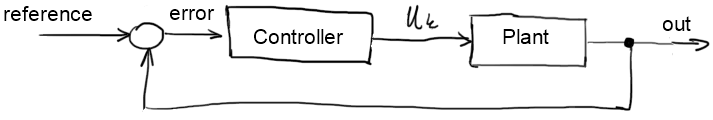
\includegraphics[width=\columnwidth]{./img/control_loop.png}
	\caption{Classical control loop.}
	\label{fig:classical_control_loop}
\end{figure}
It won't come as a surprise that the MPC follows the same general idea of the feedback loop\footnote{After all, feedback is the basic principle of cybernetics. Without feedback, there is no control.}.

Before applying the MPC algorithm, we will extend the state-space with a cross-track error \( \tilde{y}_k \) and heading error \( \tilde{\psi}_k \) variables, so that the state is now \( \bm{x}_k = \big[x_k,\ y_k,\ \psi_k,\ v_k,\ \tilde{y}_k,\ \tilde{\psi}_k \big]^\top \) and the model becomes
\begin{subequations}
\begin{align}
x_{k+1} 			&= x_k + v_k\cos(\psi_k) \mathrm{d}t \label{eq:kbm_start}\\
y_{k+1} 			&= y_k + v_k\sin(\psi_k) \mathrm{d}t \\
\psi_{k+1} 			&= \psi_k + \frac{v_k}{l_f}\delta_k \mathrm{d}t \\
v_{k+1} 			&= v_k + a_k\mathrm{d}t \\
\tilde{y}_{k+1}		&= \tilde{y}_k + v_k\sin(\tilde{\psi}_k)\mathrm{d}t \\
\tilde{\psi}_{k+1}	&= \tilde{\psi}_{k} + \frac{v_k}{l_f} \delta_k \mathrm{d}t \label{eq:kbm_end}
\end{align}
\end{subequations}
Let's think about error for a moment. 
Whenever we talk about error, we implicitly assume that there is some intended ground-truth value from which we departed - the error, therefore, expresses the difference between the desired (intended, reference) value and the actual value.
These errors arise, because the world is not perfect - actuators have their limitations, the environment is not completely predictable, there is numerical noise in calculations, communication delays on the sensor network, approximative assumptions in the modeling of the vehicle motion, etc.
The reference trajectory is supplied by the path planner module, which we haven't covered yet in the Term 3. 
For the purposes of the MPC project, the reference trajectory is created by fitting a polynomial to the supplied waypoints.

Let's define the cross-track error \( \tilde{y}_k = y_k - y^r_k \) and the heading error \( \tilde{\psi}_k = \psi_k - \psi^r_k \), where \( y^r_k \) and \( \psi^r_k \) are the reference values.
\Cref{fig:errors} shows that the reference heading at any time step \( \psi^r_k \) is the tangential angle at the point \( x_k \) of the reference trajectory \( f(x_k) \).
We know that the slope of the tangential line at \( x_k \) is given by the derivative evaluated at that point, so \( f'(x_k) = \tan(\psi^r_k) \) and thus the reference heading can be expressed as \( \psi^r_k = \arctan( f'(x_k) ) \).
The derivative \( f'(x_k) \) depends on which model we use for fitting the reference trajectory (when \( f \) is polynomial, derivatives are trivially obtained.)
\begin{figure}[h]
	\centering
	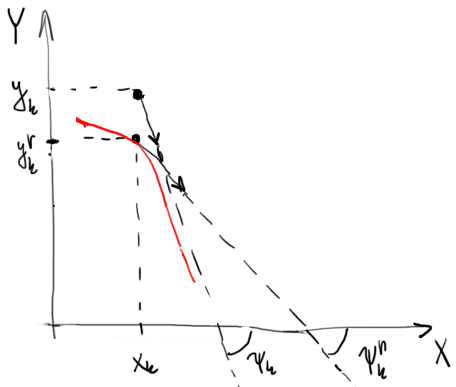
\includegraphics[width=0.5\columnwidth]{./img/errors.png}
	\caption{Cross-track error \( \tilde{y}_k = y_k - y^r_k \) and heading error \( \tilde{\psi}_k = \psi_k - \psi^r_k \). The reference track curve fit in red.}
	\label{fig:errors}
\end{figure}

Recall that, the state \( \bm{x}_k \), the control action \( \bm{u}_k \) and the reference input \( \bm{r}_k \) are defined as
\begin{align}
	\bm{x}_k &= \big[x_k,\ y_k,\ \psi_k,\ v_k,\ \tilde{y}_k,\ \tilde{\psi}_k \big]^\top \\
	\bm{u}_k &= \big[a_k,\ \delta_k\big]^\top \\
	\bm{r}_k &= \big[y^r_k,\ \psi^r_k \big]^\top
\end{align}
Let the state sequence for \( N \) time steps forward be denoted as 
\begin{equation}
	\bm{x}_{k:k+N} \triangleq \big[ \bm{x}_k,\ \bm{x}_{k+1},\ \ldots,\ \bm{x}_{k+N} \big]
\end{equation}
and analogously for sequence control actions \(  \bm{u}_{k:k+N} \) and reference inputs \( \bm{r}_{k:k+N} \).
The model predictive control computes the optimal sequence of control actions for \( N \) steps ahead by minimizing the cost function\footnote{Since \( J \) depends on the sequence of variables (which is a discretized function anyway), it is, strictly speaking, a \emph{functional}.}
\begin{equation}
u_{k:k+N} = \arg\min_{u_{k:k+N}} J(\bm{u}_{k:k+N};\, \bm{x}_{k:k+N},\ \bm{r}_{k:k+N},\, N),
\end{equation}
subject to constraints\footnote{Constraints are limits on \emph{relationships} between values.} given by the kinematic bicycle model (plant model) in \crefrange{eq:kbm_start}{eq:kbm_end} and bounds\footnote{Bounds are absolute limits on the range of values.} on the actuation variables
\begin{equation}\label{eq:mpc_actuation_bounds}
-1 \leq \alpha \leq 1 ,\qquad \SI{-25}{\degree} \leq \delta_f \leq \SI{25}{\degree}.
\end{equation}
The hyper-parameter \( N \) is referred to as the prediction horizon.

An example cost function used in MPC with our kinematic bicycle model might look something like this
\begin{equation}\label{eq:mpc_cost_simple}
	J(\bm{u}_{k:k+N};\, \bm{x}_{k:k+N},\, \bm{r}_{k:k+N},\, N) = \sum_{k=1}^{N} (\tilde{y}_k)^2.
\end{equation}
Minimizing this functional yields control actions, for which the cross-track error squared is minimal.
As you can probably guess, the heading error \( \tilde{\psi}_k \) is not reflected in the cost function, which means we can't expect it to be small after minimization.
Besides that, there are other desirable properties that we would like the resulting control sequence to have, such as minimum energy expenditure, smooth steering etc.
All of these, and more, can be incorporated by tinkering with the cost function.
A more realistic cost might look something like this
\begin{equation}\label{eq:mpc_cost_better}
	J(\bm{u}_{k:k+N};\, \bm{x}_{k:k+N},\, \bm{r}_{k:k+N},\, N) = \sum_{k=1}^{N} (\tilde{y}_k)^2 + (\tilde{\psi}_k)^2 + (\delta_k)^2+ \sum_{k=1}^{N-1} (\delta_{k+1} - \delta_k)^2.
\end{equation}
This accounts for the energy expended on the steering \( \delta_k^2 \) as well as smooth steering transitions \( (\delta_{k+1} - \delta_k)^2 \).
\Cref{fig:mpc_control_loop} outlines the model predictive control loop and role of the variables involved.
\begin{figure}[h]
	\centering
	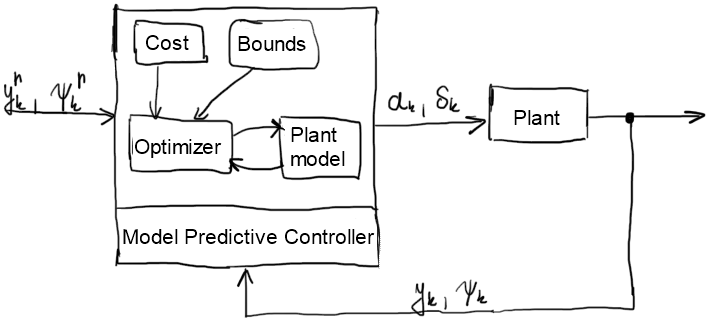
\includegraphics[width=0.8\columnwidth]{./img/mpc_control_loop.png}
	\caption{Model predictive control loop.}
	\label{fig:mpc_control_loop}
\end{figure}


\section{Implementation}
In my implementation of the MPC, I'm using the cost function 
\begin{align}\label{eq:mpc_my_cost}
	J(\bm{u}_{k:k+N}) 
	&= \sum_{k=1}^{N} w_{cte}\tilde{y}_k^2 + w_{he}\tilde{\psi}_k^2 + w_{v}\tilde{v}_k + w_{\delta}\delta_k^2  + w_{a}a_k^2 + \nonumber \\
	&\mathrel{\phantom{=}} \sum_{k=1}^{N-1} w_{\delta t}(\delta_{k+1} - \delta_k)^2 + w_a(a_{k+1} - a_k)^2,
\end{align}
where $ \tilde{v}_k = (v_k - v^r) $ and $ v^r = \SI{70}{mph} $ is the reference speed.
The weights in the cost function achieving the desired control behavior, were determined experimentally to be
\begin{align}\label{key}
w_{cte} = 1000,\ w_{he} = 2000,\  w_{v} = 2,\ w_{\delta} = 50,\ \ w_{a} = 5,\ w_{\delta t} = 2000,\ w_{\delta a} = 10.
\end{align}
During the experiments, I initially stuck with prediction horizon $ N = 10 $, but eventually went down to $ N = 7 $.
As that didn't give satisfactory car behavior I went up to $ N = 8 $, which exhibited the best control behavior at the chosen reference speed and seemed like a good trade-off between the computational load and the quality of the result.
I saw no need to fiddle with the discretization period, so I stuck to $ \mathrm{d}t = \SI{0.1}{s} $.

The reference car position $ y^r $ and heading $ \psi^r $ are determined from the 3rd-degree polynomial fit to the waypoints.
The polynomial model and it's derivative are given by
\begin{align}\label{eq:trajectory_polynomial}
	f(x_k) 	&= a_3x_k^3 + a_2x_k^2 + a_1x_k + a_0, \\
	f'(x_k) &= 3a_3x_k^2 + 2a_2x_k + a_1.
\end{align}
Since we are fitting the model in the car's coordinates, where $ x_k = 0,\ y_k = 0 $.
Using the reasoning from the previous sections, the reference position and heading are given by
\begin{align}\label{}
y^r_k 		&= f(0) = a_0, \\
\psi^r_k	&= \arctan(f'(0)) = \arctan(a_1),
\end{align}
and the cross-track error and heading error thus become
\begin{align}\label{}
	\tilde{y}_k 	&= y_k - y^r_k = -a_0,	\\
	\tilde{\psi}_k 	&= \psi_k - \psi^r_k = -\arctan(a_1).
\end{align}
So, at every time step, the optimization is started with the initial state (which is part of the constraints given by the kinematic bicycle model)
\begin{equation}\label{}
	\bm{x}_k = \left[ 0,\ 0,\ 0,\ v,\ \tilde{y}_k,\ \tilde{\psi}_k \right].
\end{equation}



% ==========================
\bibliographystyle{plainnat}
\bibliography{refereces}

\end{document}